本研究では,深層学習を用いて上田研のテーマとする「優美さ」を対象に,
深層学習を使用した場合の結果を得て,それを先行研究らと比較することを目的とした.

まず,入力された動画を[優美なダンス,普通のダンス,その他の動作]に分類するネットワークを作成した.
ネットワーク内での分類手順として
\begin{enumerate}
  \item 動画に特別な編集を施す
  \item 作成したネットワークに通す
  \item 配列長3の二値データを得る
\end{enumerate}
のような順序で分類した.
次に,得た結果を判断根拠可視化手法らで検証した.先行研究との差分の検証を論ずることを目標とした.
最後に,それらを踏まえて先行研究,本研究の改善点,成功点を述べた.

\begin{figure}[b]
  \begin{center}
    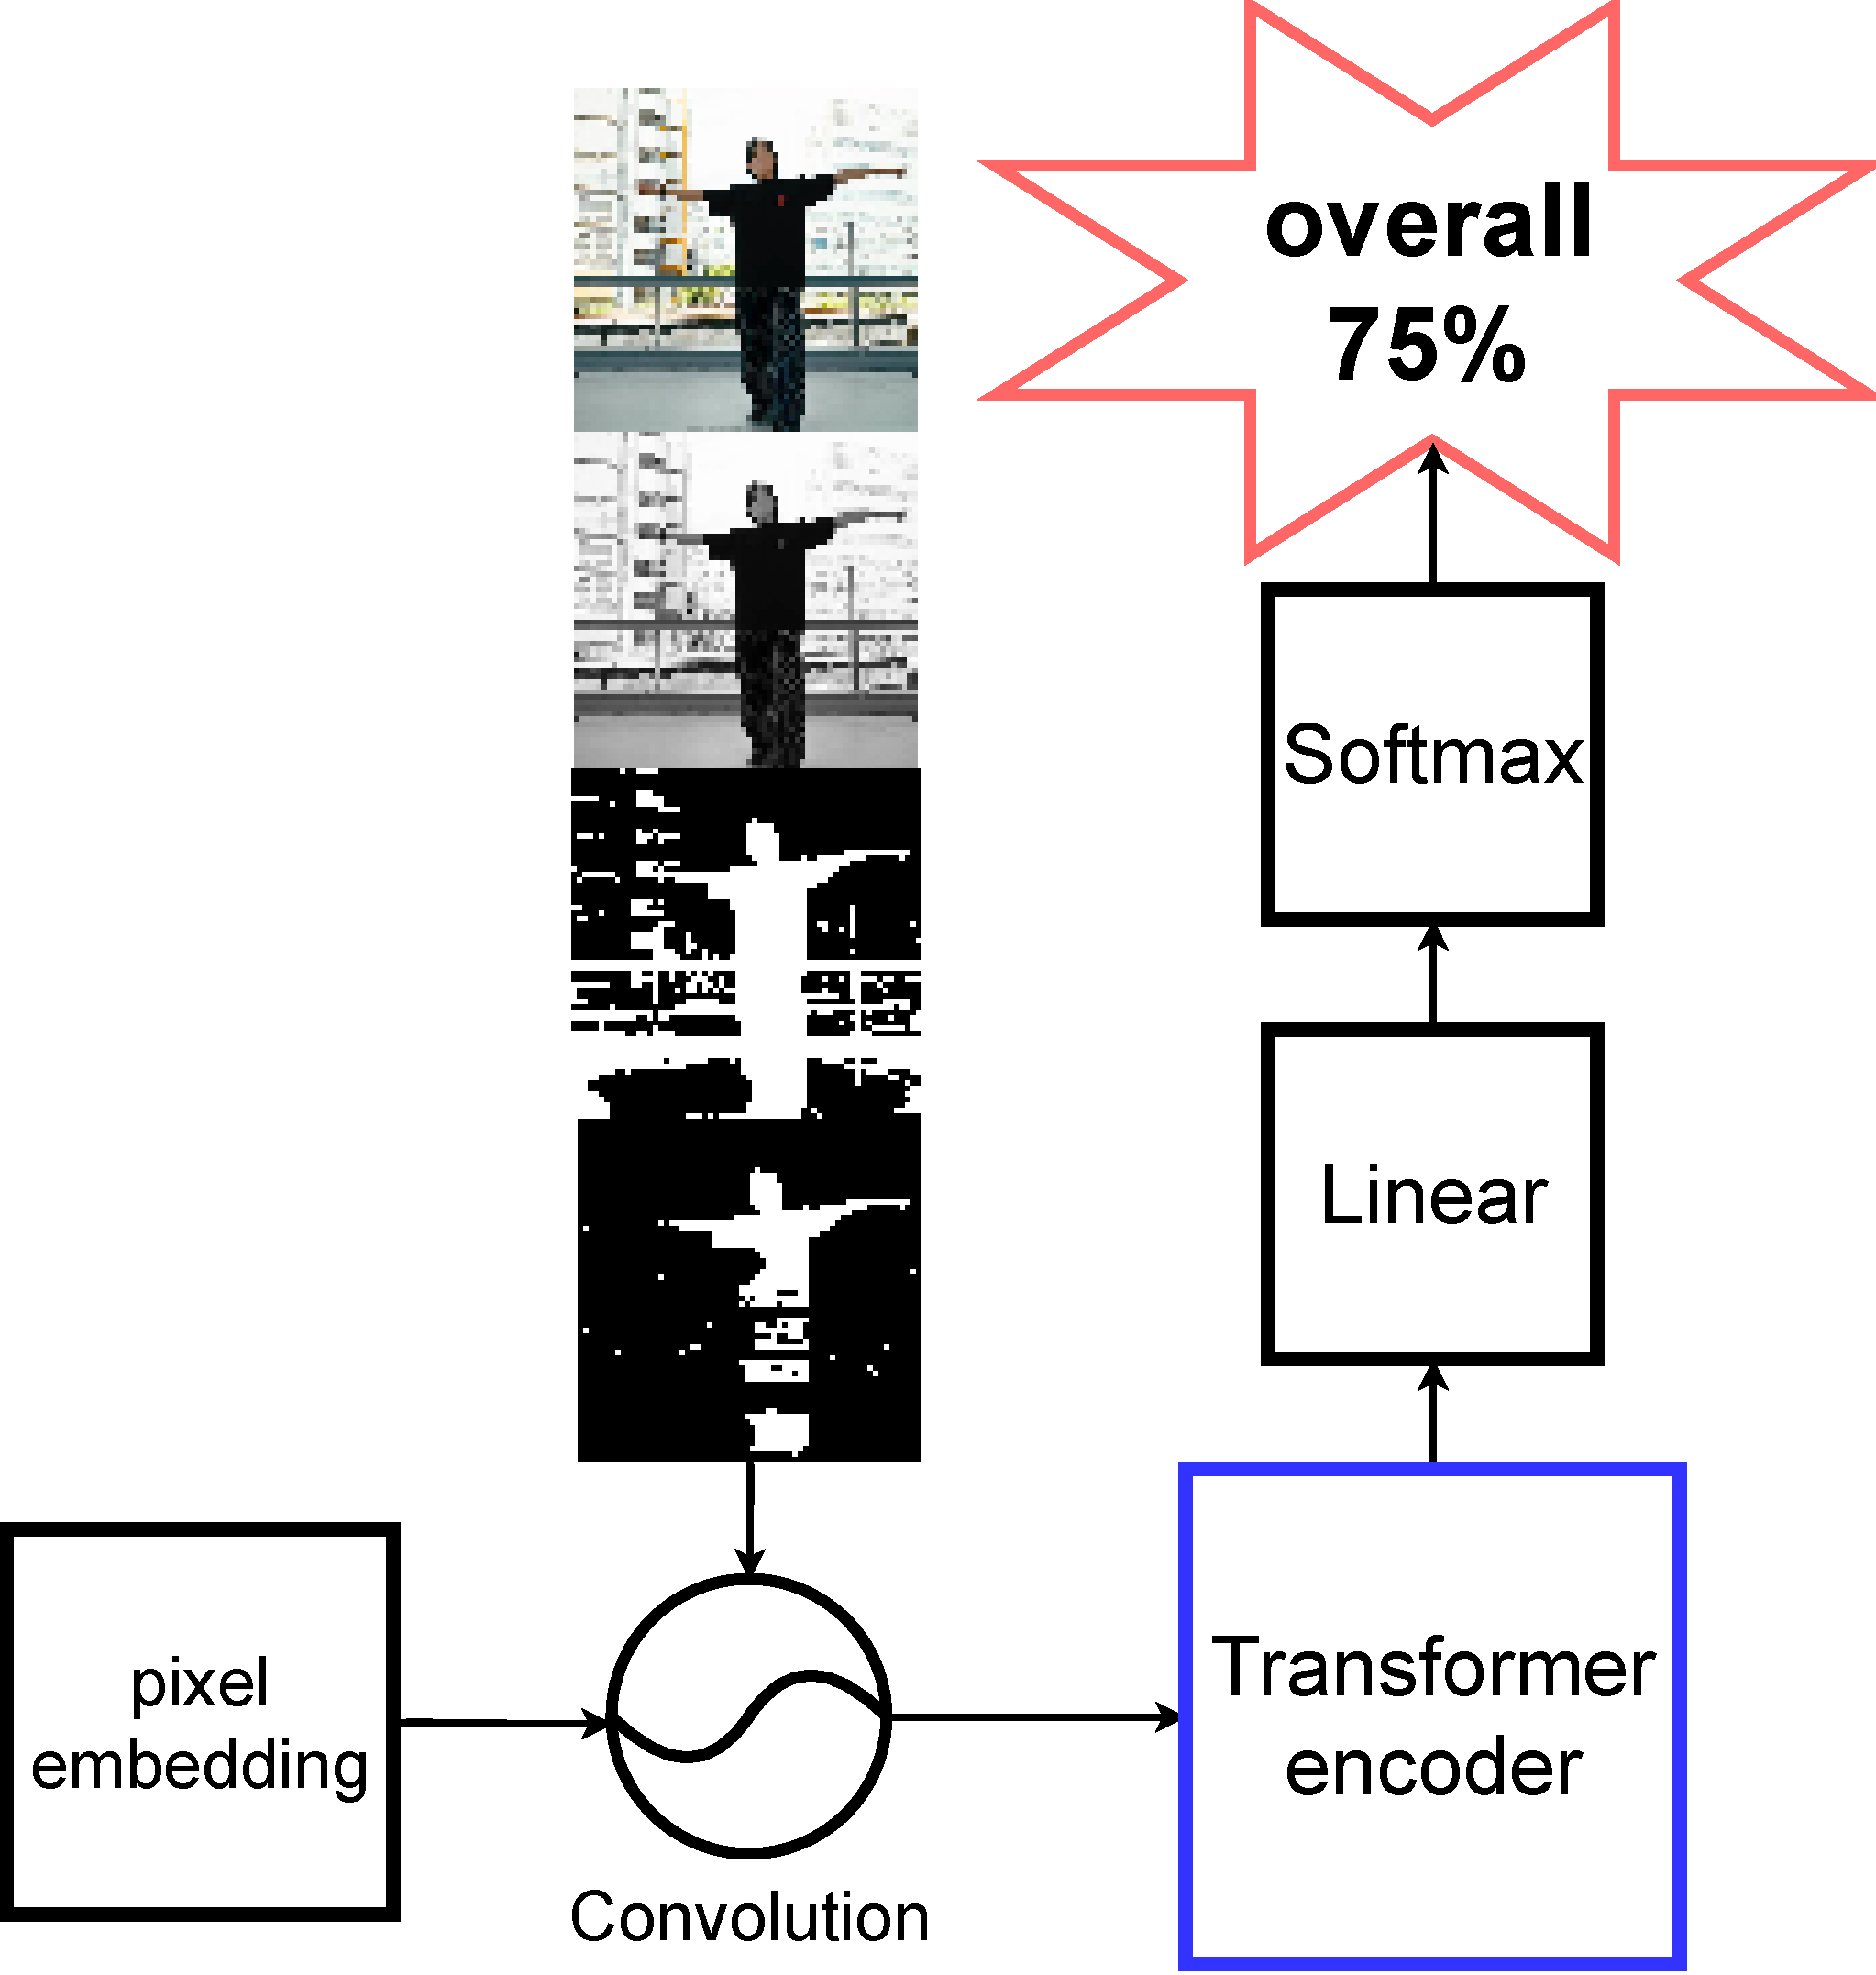
\includegraphics[width=80mm]{images/chart/easy_chart.pdf}
  \end{center}
  \caption{モデル概要}
  \label{easy_chart}
\end{figure}